\chapter{Система Кумир}

\section{Введение}
\subsection{Общие сведения}

Система Кумир --- позволяет создавать, отлаживать и выполнять программы на универсальном языке программирования Кумир.

Кумир --- учебная система. Она сводит к минимуму «накладные расходы» на освоение, имеет развитую систему диагностики ошибок, средства, позволяющие ученику следить за выполнением программы и~т.~п. Ученик, никогда ранее не программировавший, может начать писать и выполнять алгоритмически относительно сложные программы через 1--2 часа после первого знакомства с Кумиром. В то же время система Кумир позволяет создавать достаточно большие и сложные программы (сотни строк).

Во время редактирования программы система Кумир после каждого перевода курсора на новую строку автоматически производит синтаксический разбор и сообщает о найденных ошибках.

Система Кумир включает графические исполнители Робот и Чертежник, которыми можно управлять из программы (а Роботом кроме того можно управлять вручную). 

\subsection{Основная программа}

В каждый момент пользователь работает только с \emph{одной Кумир-программой}, которую мы называем \emph{основной} (в данный момент) программой системы Кумир. Текст основной программы представлен в \emph{рабочем окне} (редакторе) системы Кумир (см.~\ref{windows}). Пользователь может прочитать текст основной программы из файла и поместить этот текст в редактор, редактировать текст и сохранить подготовленный текст в файл. Именно к основной программе относятся команды системы Кумир на выполнение.

Во время сеанса работы, кроме текста основной программы пользователю могут потребоваться и другие связанные с ней объекты --- вспомогательные программы, написанные на Кумире (т.~н.~внешние исполнители), файлы с входными данными для основной программы и результатами ее работы, различные описания и~т.~п. Система Кумир имеет средства, облегчающая работу с этими вспомогательными объектами. 

\subsection{Язык Кумир. Исполнители}

Язык Кумир --- универсальный язык программирования, его прототипом послужил «школьный язык программирования» разработанный А.~П.~Ершовым в первой половине 80-х годов ХХ~века. В дополнение к обычным для универсальных языков программирования возможностям, Кумир имеет средства управления \emph{исполнителями}. Говоря неформально, исполнитель – это устройство, которое может выполнять определенный набор действий. Действие может совершаться над внешними для исполнителя данными (\emph{параметрами действия}) и/или над присущими исполнителю внутренними для него данными (\emph{обстановкой исполнителя}).

Примером исполнителя может служить Робот. Его обстановка --- это прямоугольник, разделенный на квадратные клетки. Размер прямоугольника может варьироваться. Каждой клетке приписаны числовые характеристики --- «температура» и «радиация». Робот может «измерять» значения этих величин, а также передвигаться по клеткам по горизонтали и вертикали (действия \textsf{влево}, \textsf{вправо}, \textsf{вперед}, \textsf{назад}). Границы между некоторыми клетками непроходимы для Робота (там стоят «стены»), Робот умеет выполнять проверки \textsf{слева стена}, \textsf{справа стена} и~т.~п. При попытке «пройти через стену» в любом направлении возникает ситуация \emph{отказ}.

Робот --- пример встроенного исполнителя. Пользователь также может описать свои исполнители на языке Кумир.

\subsection{Сеанс работы системы Кумир. Состояния системы}

Работа пользователя  в системе Кумир состоит в:
\begin{itemize}
\item подготовке программы к выполнению (редактирование, загрузка/сохранение программы, настройка параметров системы и~т.~п.);
\item выполнении программы (в обычном или отладочном режиме);
\item просмотре (анализе) результатов работы программы (окончательных или промежуточных).
\end{itemize}

В зависимости от выполняемого действия, система Кумир находится в одном из четырех возможных состояний:
\begin{itemize}
\item РЕДАКТИРОВАНИЕ
\item ВЫПОЛНЕНИЕ
\item АНАЛИЗ РЕЗУЛЬТАТОВ (или просто АНАЛИЗ)
\item ПАУЗА
\end{itemize}

Состояние системы накладывает естественные ограничения на возможность выполнения различных действий. Например, во время выполнения программы нельзя изменять ее текст. 

Смысл двух первых состояний ясен из их названия.  В состояние АНАЛИЗ  система переходит после окончания выполнения программы (нормального или аварийного). В этом состоянии пользователю доступны все рабочие сообщения программы --- для просмотра и анализа. Любое действие по изменению текста программы сбрасывает эти рабочие сообщения и переводит систему в состояние РЕДАКТИРОВАНИЕ. В состояние ПАУЗА система переходит в случае остановки во время выполнения (при вызове встроенной функции \textsf{\textbf{\mbox{пауза}}} или после очередного шага при выполнении программы «по шагам», см.~\ref{menurun}). Схема возможных переходов между состояниями выглядит так:
\begin{itemize}
\item РЕДАКТИРОВАНИЕ $\to$ ВЫПОЛНЕНИЕ
\item ВЫПОЛНЕНИЕ  $\to$ \{АНАЛИЗ, ПАУЗА\}
\item ПАУЗА $\to$ \{ВЫПОЛНЕНИЕ,  АНАЛИЗ\}
\item АНАЛИЗ  $\to$ \{ВЫПОЛНЕНИЕ,  РЕДАКТИРОВАНИЕ\}
\end{itemize}

\subsection{Запуск системы Кумир}

Запуск системы Кумир может быть выполнен стандартными средствами операционной системы:
\begin{itemize}
\item командной строкой;
\item щелчком по пиктограмме системы Кумир;
\item щелчком по пиктограмме файла с Кумир-программой (файл с расширением .kum).
\end{itemize}

\subsubsection{Дополнительные ключи запуска}
\begin{itemize}
\item \textbf{-z}
\begin{itemize}
\item Формат вызова: \textsf{kumir -z \textit{путь}}

Сохранять настройки системы Кумир не в реестре, а в INI-файле. Файл \textit{kumir.ini} должен располагаться в директории \textit{путь}. Если в указанной директории этого файла нет, то он создается, а настройки системы принимаются по умолчанию.

\item Формат вызова: \textsf{kumir -z \textit{имя\_файла}}

Сохранять настройки системы Кумир не в реестре, а в INI-файле \textit{имя\_файла}. Если этого файла не существует, то он создается, а настройки системы принимаются по умолчанию.
\end{itemize}
\end{itemize}

\section{Рабочее окно и другие окна системы Кумир}
\label{windows}

\subsection{Главное окно системы Кумир}

После запуска Кумира на экране появляется \emph{главное окно системы Кумир}. Главное окно открывается при начале сеанса работы системы Кумир и закрывается в момент окончания сеанса работы. Иногда мы будем называть это окно \emph{рабочим}, т.~к.~основная работа с системой происходит именно в этом окне.

Главное окно системы Кумир имеет стандартный вид. Вверху окна расположены заголовок окна, главное меню и  панель инструментов; снизу --- строка состояния. Заголовок окна содержит полное имя файла, из которого была загружена основная программа. Строка состояния используется для вывода сообщений, показа положения курсора, состояния системы и~т.~п.

При работе с окном доступны стандартные возможности управления окнами: окно можно свернуть-развернуть, сжать-растянуть, передвинуть и~т.~п. При закрытии окна его параметры (например, размеры и положение) запоминаются; при следующем запуске окно открывается с теми же параметрами.

\subsection{Структура главного окна}

Собственно окно разбито на две \emph{основные области}: \emph{рабочую} область (вверху) и область \emph{ввода-вывода} (внизу).

В рабочей области располагается основная программа --- программа, с которой в данный момент работает система Кумир. При этом рабочая область делится на две части: область \emph{программы} (слева) и область \emph{построчных сообщений}  (справа). Область построчных сообщений  аналогична \emph{«полям»} в ученических тетрадях. В эту область при подготовке программы выводятся сообщения об ошибках,  найденных в каждой строке, а при выполнении --- сведения о значениях переменных, присваиваемых в  строке.

Строки в области программы  и области построчных сообщений синхронизированы: при прокрутке текста в области программы синхронно прокручиваются и сообщения. Относительные размеры (по горизонтали) области программы и «полей», а также размер области ввода-вывода по вертикали могут меняться пользователем. 

Как по горизонтали, так и по вертикали виртуальный размер всех текстов не ограничены, поддерживается прокрутка.

\subsection{Меню главного окна}

Меню главного окна (главное меню системы Кумир) содержит восемь пунктов:
\begin{itemize}
\item	Программа
\item	Редактирование
\item	Вставка
\item	Выполнение
\item	Инструменты
\item	Робот
\item	Чертежник
\item	Инфо
\end{itemize}

Каждому из этих пунктов соответствует свое раскрывающееся меню. Как правило, действие, для которого есть команда в главном меню,  может быть выполнено также с помощью аккорда клавиш и/или инструментальной кнопки. В последнем случае нужный аккорд или пиктограмма приводятся рядом со строкой раскрывающегося меню. 

Меню «Программа», «Редактирование» и «Вставка» описаны в~\ref{preparing}; меню «Выполнение» --- в~\ref{run}; меню «Инструменты» --- в~\ref{tools}. Отметим, что меню «Инструменты» не обязательно при первом знакомстве с системой Кумир.

Меню «Робот» и «Чертежник» посвящены встроенным графическим исполнителям системы Кумир, они описаны в отдельных руководствах.

Меню «Инфо» содержит сведения о версии системы Кумир, а также обеспечивает доступ к руководствам:
\begin{itemize}
\item по алгоритмическому языку Кумир;
\item по использованию системы Кумир (настоящее руководство);
\item по работе с исполнителем Робот;
\item по работе с исполнителем Чертежник.
\end{itemize}

Все эти руководства подготовлены в виде pdf-файлов и могут просматриваться стандартными средствами как в ходе сеанса работы системы Кумир, так и автономно.

\subsection{Инструментальные кнопки}

Инструментальные кнопки (за исключением двух) расположены на панели инструментов, которая расположена под главным меню. Эта панель разбита на области, разделенные двойным пунктиром; порядок областей соответствует пунктам главного меню. Каждая кнопка снабжена всплывающей подсказкой, текст подсказки совпадает с текстом в раскрывающемся меню.

\subsection{Область ввода-вывода}
\label{io}

Область снизу главного окна системы Кумир предназначена для отображения вывода программы и для ввода данных в программу.

После каждого выполнения программы в область ввода-вывода добавляется горизонтальная линия. Таким образом, выводы отдельных запусков программ всегда разделены между собой.

Каждый вывод программ содержит в своем начале и конце специальные строки. Подробнее об этом см.~\ref{io-run}.

Слева снизу области ввода-вывода находятся две кнопки управления ею: <<Сохранить область вывода>> и <<Очистить область вывода>>. Они также дублируются в командах главного меню <<Инструменты>>. Кнопка очистки просто очищает область вывода, а при нажатии на кнопку сохранения появляется подменю:
\begin{itemize}
\item Сохранить все
\item Сохранить только последний вывод
\item Сохранить выделенный текст
\end{itemize}
Назначение этих пунктов интуитивно понятно. Вывод сохраняется в текстовый файл.

\section{Подготовка программы. Меню «Программа», «Редактирование», «Вставка»}
\label{preparing}

\subsection{Меню «Программа». Файлы, хранящие Кумир-программы}
\label{menufile}

Меню «Программа» обеспечивает работу с файлами, в которых хранятся Кумир-прог\-рам\-мы, эти файлы имеют расширение .kum. Меню содержит следующие пункты:
\begin{itemize}
\item Новая программа
\item Недавние программы
\item Открыть программу
\item Сохранить программу
\item Сохранить программу как\dots
\item Передать программу\dots
\item Печать программы
\item Выход
\end{itemize}

Эти пункты имеют стандартный для современных оконных систем смысл. Для пункта «Сохранить» есть инструментальная кнопка.

Пункт <<Передать программу\dots>> предназначен для передачи текста программы из редактора Кумира в какой-либо дополнительный модуль (например, в конвертор).

\subsection{Редактирование программы}

Редактор системы Кумир обеспечивает стандартные средства редактирования текстов: ввод символов в режиме вставки или замены, удаление символов, выделение~/ копирование~/ вставку~/ удаление фрагмента текста, «откатку» (отмену последних действий) и «накатку» (отмену откатки), поиск по тексту и~т.~п. Эти действия можно выполнять как в непосредственном режиме, так и с помощью меню «Редактирование». Кроме того, редактор программ системы Кумир предоставляет пользователю дополнительные возможности, ориентированные на специфику языка Кумир.

Редактор программ всегда использует шрифт, в котором все символы имеют одинаковую ширину. Какой именно это будет шрифт и его размер, пользователь может установить на вкладке «Внешний вид» диалогового окна «Настройки». Подробнее об этом см.~\ref{settings-view} 

\subsection{Меню «Редактирование»}

Меню «Редактирование» содержит следующие строки:
\begin{itemize}
\item		Отменить
\item		Отменить отмену
\item		Вырезать
\item		Копировать
\item		Вставить
\item		Найти и заменить
\item		Закомментировать
\item		Раскомментировать
\item		Перехватывать команды Пульта
\item		Макросы
\end{itemize}

Первые шесть строк имеют стандартный смысл и могут быть выполнены с помощью стандартных аккордов, для них (кроме «Найти и заменить») предусмотрены инструментальные кнопки.

Команда «Закомментировать» добавляет знак комментария \textbf{\textsf{|}} в начало каждой выделенной (хотя бы частично) строки. Команда «Раскомментировать» удаляет знак комментария из начала каждой выделенной строки. Если в начале выделенной строки не было знака комментария, то содержимое этой строки не меняется. Для команд «Закомментировать» и «Раскомментировать» предусмотрены инструментальные клавиши.

Команда «Перехватывать команды Пульта» связана с работой встроенного исполнителя Робот и позволяет вставлять в программу команды этого исполнителя. Подробнее --- см. руководство по исполнителю Робот.

Строка «Макросы» описана ниже.

\subsection{Макросы}

Строка «Макросы» меню «Редактирование» позволяет запомнить нужную пользователю последовательность действий (\emph{макрос}), а затем выполнить всю эту последовательность, нажав клавишу \textsf{Esc}, а потом --- еще одну (выбранную пользователем) клавишу. Каждому макросу, таким образом, соответствуют:
\begin{itemize}
\item выполняемая последовательность действий редактирования;
\item клавиша, используемая при вызове этой последовательности.
\end{itemize}

Кроме того, макросу соответствует условное \emph{имя}, используемое при редактировании набора макросов. Определенные таким образом макросы сохраняются от сеанса к сеансу работы системы Кумир, т.~е.~пользователь может создать свою собственную библиотеку макросов. 

Строка «Макросы» приводит к появлению вспомогательного меню, включающего 3 пункта:
\begin{itemize}
\item Начать запись макроса
\item Завершить запись макроса
\item Список макросов
\end{itemize}

После этих пунктов перечислены определенные в данный момент макросы. Для вызова макроса (вместо использования клавиши \textsf{Esc} и клавиши, определенной пользователем) достаточно щелкнуть левой кнопкой мыши по строке этого макроса.

Из двух первых пунктов вспомогательного меню «Макросы» в каждый момент активен лишь один. Обычно, активен пункт «Начать запись макроса», а после того, как запись макроса начата, активным становится пункт «Завершить запись макроса». После того, как начата запись макроса, система Кумир запоминает все действия пользователя по редактированию программы (одновременно эти действия выполняются).  По сигналу об окончании записи макроса, появляется диалоговое окно, предлагающее определить для нового макроса имя и клавишу вызова. 

Пункт «Список макросов» приводит к появлению вспомогательного окна, содержащего список определенных пользователем макросов. С помощью этого окна пользователь может удалить любой макрос или изменить его имя и клавишу.

\emph{Примечание.} По техническим причинам в окне определения макросов клавиши обозначаются заглавными латинскими буквами. При вызове макроса раскладка клавиатуры (рус/лат, большие/маленькие буквы) не важна.

\subsection{Меню «Вставка»}

В этом меню описаны встроенные в систему макросы, обеспечивающие ввод в текст программы стандартных конструкций. Эти макросы не могут быть удалены или отредактированы или отредактированы пользователем. Меню «Вставка» позволяют вводить в текст программы следующие конструкции, для каждой конструкции указана соответствующая клавиша.

\subsection{Возможности редактора, ориентированные на язык Кумир}

Редактор системы Кумир ориентирован именно на работу с программами на языке Кумир. Это проявляется различными способами, которые представлены ниже.

\subsubsection{Временное переключение раскладки клавиатуры}
В редакторе Кумир есть возможность ввода символов из другой (русской или латинской раскладки), не переключая ее.
Для этого необходимо вводить символы с нажатой клавишей "Alt".

Например, при активной русской раскладке клавиатуры, нажимая последовательно клавиши: \textsf{ц}, \textsf{е}, \textsf{л},
 \textsf{пробел}, \textsf{Alt+ш}, получим текст: \textbf{\textsf{цел}} \textsf{i}.
 
Кроме того, для некоторых часто используемых последовательностей, зарезервированы сочетания клавиш (в любой раскладке клавиатуры):
\begin{itemize}
\item \textsf{Alt+=} -- вводит последовательность символов присваивания \textbf{\textsf{:=}}
\item \textsf{Alt+1} -- вводит символ комментария \textbf{\textsf{|}}
\end{itemize}
	
\subsubsection{Синтаксический разбор и сообщения об ошибках}

Всякий раз, когда курсор переходит на новую строку, происходит синтаксический разбор программы (всей программы, а не только этой строки). При этом отмечаются ошибки (если они есть), а также происходит разметка текста программы, облегчающая работу с ним:
\begin{itemize}
\item различные компоненты программы выделяются различными цветами и видами шрифта;
\item в программе расставляются отступы так, чтобы части одной конструкции (\textbf{\textsf{нач-кон}}, \textbf{\textsf{нц-кц}} и~т.~п.) оказались друг под другом.
\end{itemize}
	
Сообщения об ошибках выводятся в область построчных сообщений (на «поля»), каждое сообщение --- напротив той строки, в которой обнаружена ошибка. Место ошибки подчеркивается красным. Если в строке найдено более одной ошибки, то диагностируется только одна (первая слева).

\subsubsection{Отступы}

Отступы изображаются точками в левой части строки, при синтаксическом разборе эти точки игнорируются. Размер отступа (количество позиций на один отступ) можно установить с помощью меню <<Настройки>> $\to$ <<Внешний вид>>.

Пользователь может поместить курсор в область отступов с помощью мыши или стрелок и передвигать его с помощью стрелок. Однако, для изменений эти области заблокированы. Если нажать какую-нибудь клавишу, отличную от стрелки, то произойдет следующее. Если это символьная клавиша, то курсор будет передвинут в первую «значащую» позицию строки и там будет выведен указанный символ. Клавиша \textsf{Delete}, не меняя текста,  переведет курсор в первую значащую позицию строки. Клавиша \textsf{BackSpace}, не меняя текста,  переведет курсор в конец предыдущей строки.

\subsubsection{Выделение цветом и шрифтом}
\label{highlight}

Различные компоненты текста программы выделяются цветом и видом шрифта (жирность, курсив). К таким компонентам относятся:
\begin{itemize}
\item		Типы величин
\item		Значения (числовые и логические)
\item		Строковые значения
\item		Имена исполнителей
\item		Имена алгоритмов
\item		Строки описаний алгоритмов (начинающиеся со знака \#)
\item		Комментарии
\end{itemize}

Рекомендуется также выводить курсивом латинские буквы в именах, чтобы не путать их с близкими по начертанию русскими буквами.

Пользователь сам может настроить выбор цветов и свойств шрифта, используя панель «Настройки>> $\to$ <<Подсветка кода». Для настройки цвета нужно щелкнуть правой кнопкой по цветовому квадратику.

\subsubsection{Угадывание имен алгоритмов}

Система Кумир облегчает пользователю ввод длинных имен алгоритмов. Если набрать несколько первых букв имени алгоритма, а потом аккорд \textsf{Ctrl-пробел} (кроме ОС~Mac) или \textsf{Tab} (кроме ОС~MS~Windows), то:
\begin{itemize}
\item если эти буквы однозначно определяют имя алгоритма, то введенное начало будет расширено до этого имени;
\item если есть несколько вариантов, то пользователю будет предложено выбрать из них;
\item если алгоритма с указанным началом нет, ничего не произойдет.
\end{itemize}

\section{Выполнение программ. Меню «Выполнение»}
\label{run}

\subsection{Основные сведения}

В этом разделе мы напоминаем необходимые сведения о языке Кумир. Подробнее --- см.~описание языка Кумир.

Выполнение программы на языке Кумир состоит в том, что последовательно выполняются:
\begin{itemize}
\item инструкции \textsf{использовать\dots} (если они есть, см.~\ref{use});
\item вступление к программе (если оно есть);
\item основной алгоритм (если он есть).
\end{itemize}

Выполнение программы происходит по шагам. Один шаг выполнения состоит в:
\begin{itemize}
\item выполнении \emph{простой} команды или 
\item проверке условия в составной команде (например, \textsf{\textbf{если}\dots}) или 
\item выполнении вспомогательного действия в составной команде (например, обработке ключевого слова \textsf{\textbf{кц}}).
\end{itemize}

При развернутой записи программы каждый шаг выполнения соответствует одной строке программы. Однако, возможна и более компактная запись, при которой одна строка соответствует нескольким шагам выполнения.

Особую роль играют вызовы вспомогательных алгоритмов, представленных в текущей программе. По желанию пользователя, такой вызов может трактоваться как один шаг (крупный «ШАГ»). В то же время, можно и «войти внутрь вызова». Тогда очередной шаг (мелкий «шаг») будет состоять только в выполнении строки-заголовка, а выполнение всего вызова будет рассматриваться как цепочка мелких шагов.

Выполнение программы завершается \emph{нормально}, если выполнена строка \textsf{\textbf{кон}} основного алгоритма или выполнены все строки вступления (если основного алгоритма нет). Кроме того, выполнение может завершиться аварийно --- если произошла ошибка при выполнении одной из команд или пользователь остановил выполнение командой «Прервать» (см.~ниже). В случае аварийного завершения работы программы в поле ввода-вывода выводится сообщение о причинах аварии.

\subsection{Выполнение программы и состояния системы Кумир}

Напомним, что система Кумир может находиться в таких состояниях:
\begin{itemize}
\item РЕДАКТИРОВАНИЕ: происходит подготовка программы, выполнения нет.
\item ВЫПОЛНЕНИЕ:  происходит выполнение программы, редактирование текста программы запрещено.
\item ПАУЗА: выполнение программы приостановлено, но может быть продолжено; редактирование текста программы запрещено.
\item АНАЛИЗ: выполнение завершено, однако все сообщения программы доступны для наблюдения и анализа; по любому действию в области программы рабочего окна, система переходит в состояние РЕДАКТИРОВАНИЕ.
\end{itemize}

Переход в состояние ВЫПОЛНЕНИЕ возможен из состояний:
\begin{itemize}
\item РЕДАКТИРОВАНИЕ, АНАЛИЗ (с помощью команд «Выполнить непрерывно», «Неп\-ре\-рыв\-но без показа на полях», «ШАГ», «шаг»);
\item ПАУЗА (с помощью команд «Выполнить непрерывно», «Непрерывно без показа на полях», «ШАГ», «шаг», «До конца алгоритма»).
\end{itemize}

Из состояния ВЫПОЛНЕНИЯ система Кумир может перейти в состояния: 
\begin{itemize}
\item АНАЛИЗ, если выполнение программы завершено (нормально или аварийно);
\item ПАУЗА (при выполнении команды \textsf{\textbf{ввод}} или встроенных функций \textsf{\textbf{пауза}} и \textsf{\textbf{клав}} (см.~описание языка Кумир), или при выполнении по шагам, см.~ниже).
\end{itemize}

\subsection{Вывод значений на поля}
\label{diagnost}

Как правило, при выполнении Кумир-программы, на поля выводятся значения, присваиваемые величинам и результаты проверок. Вывод значений на поля производится при выполнении следующих команд:
\begin{itemize}
\item команда присваивания (пример сообщения: \textsf{н=5})
\item команда ввод (пример сообщения: \textsf{н=5})
\item заголовок цикла «для» (пример сообщения: \textsf{н=5}) 
\item заголовок цикла «раз» (пример сообщения: \textsf{5 раз})
\item команды контроля выполнения (\textsf{\textbf{утв}}, \textsf{\textbf{дано}}, \textsf{\textbf{надо}}) (примеры сообщений: \textsf{да}, \textsf{нет}) 
\item конструкции проверки условий (\textsf{\textbf{пока}}, \textsf{\textbf{если}}, \textsf{\textbf{при}}, \textsf{\textbf{кц\_при}}) (примеры сообщений: \textsf{да}, \textsf{нет}) 
\end{itemize}

Если в одной строке записано несколько команд, то на поля выводится несколько сообщений, разделенных точкой с запятой.

\subsection{Выполнение первого алгоритма с параметрами}
\index{первый алгоритм}
\label{FirstAlg}

Первый алгоритм может иметь параметры, типами который являются простые величины (\textbf{цел}, \textbf{вещ}, \textbf{лог}, \textbf{сим}, \textbf{лит}).

Перед выполнением первого алгоритма, система КуМир запрашивает у пользователя значения всех \textbf{арг} и \textbf{аргрез} параметров,
а после его выполнения - выводит значения \textbf{рез} и \textbf{аргрез} параметров.

Если алгоритм является функцией (то есть возвращает некоторое значение), то после его выполнения также выводится возвращаемое значение.

\emph{Пример.}\\
{
\sffamily
\textbf{алг} \textbf{лит} алгоритм(\textbf{вещ} а, \textbf{рез цел} р)\\
\textbf{нач}\\
\otstup р := int(а)\\
\otstup знач := вещ\_в\_лит(а)\\
\textbf{кон}
}

\emph{Выполнению этого алгоритма соответствует программа:}\\
{
\sffamily
\textbf{алг}\\
\textbf{нач}\\
\otstup \textbf{вещ} а\\
\otstup \textbf{цел} р\\
\otstup \textbf{цел} результат\_алгоритм\\
\otstup \textbf{вывод} \lq\lq Введите а: \rq\rq\\
\otstup \textbf{ввод} а\\
\otstup результат\_алгоритм := алгоритм(а, р)\\
\otstup \textbf{вывод} \lq\lq Значение функции = \rq\rq, результат\_алгоритм, \textbf{нс}\\
\otstup \textbf{вывод} \lq\lq р = \rq\rq, р, \textbf{нс}\\
\textbf{кон} \\
\\
\textbf{алг} \textbf{лит} алгоритм(\textbf{вещ} а, \textbf{рез цел} р)\\
\textbf{нач}\\
\otstup р := int(а)\\
\otstup знач := вещ\_в\_лит(а)\\
\textbf{кон}
}


\subsection{Меню «Выполнение»}
\label{menurun}

Действия, связанные с выполнением основной программы, выполняются с помощью меню «Выполнение». В этом меню шесть пунктов. Для всех этих пунктов предусмотрены аккорды и инструментальные кнопки.

\subsubsection{Выполнить непрерывно}

Начинает (при состоянии системы РЕДАКТИРОВАНИЕ или АНАЛИЗ) или продолжает (при состоянии системы ПАУЗА) выполнение программы. Программа выполняется «непрерывно», т.~е.~без остановок между шагами. Выполнение программы может быть завершено (нормально, аварийно или по команде «Прервать») или приостановлено, если в ходе выполнения будет выполняться команда \textsf{\textbf{ввод}}, либо одна из встроенных функций \textsf{\textbf{пауза}} или \textsf{\textbf{клав}}.

Во время выполнения на поля выводятся вычисляемые значения величин и условий (см.~\ref{diagnost}).

\subsubsection{Непрерывно без показа на полях}

Аналогично «Выполнить непрерывно» --- но без вывода на поля вычисляемых значений величин и условий.

\subsubsection{ШАГ}

Выполняет один ШАГ программы и переходит в режим ПАУЗА. Допускается использование в состояниях РЕДАКТИРОВАНИЕ, АНАЛИЗ, ПАУЗА. При запуске в состоянии РЕДАКТИРОВАНИЕ и АНАЛИЗ «проскакивает» строки \textsf{\textbf{использовать}\dots} и останавливается перед выполнением первой строки вступления основной программы (если оно есть) или перед выполнение \textsf{\textbf{алг}}-строки основного алгоритма. Выполнение команды вызова алгоритма-процедуры трактует как один ШАГ.

\subsubsection{шаг}

Аналогично команде «ШАГ». Отличие состоит в трактовке команды алгоритма-процедуры и вычислении значении алгоритма-функции (если они представлены в текущей программе). В этих случаях очередным шагом будет выполнение строки-заголовка вспомогательного алгоритма. В дальнейшем команда «шаг» или «ШАГ» приведет к выполнению очередного шага внутри выполняемого вспомогательного алгоритма.

\subsubsection{До конца алгоритма}

Допускается использование только в состоянии ПАУЗА. Программа выполняется непрерывно, но останавливается на первой встретившейся строке \textsf{\textbf{кон}} (как будто перед ней стоит вызов функции \textsf{\textbf{пауза}}).

\subsubsection{Прервать}

Прерывает выполнение программы. Допускается использование только в состояниях ВЫПОЛНЕНИЕ и ПАУЗА.

\subsection{Отображение выполнения в области ввода-вывода}
\label{io-run}

В начале выполнения программы в поле ввода вывода выводится строка-заголовок вида:\\
\texttt{> 16:39:48 - Новая программа* - Начало выполнения}

Далее под этой линией появляются все сообщения, выводимые программой (включая эхо ввода, см.~ниже). В конце работы программы выводится итоговая строка и линия-разделитель. Предусмотрено 3 вида заключительной строки:
\begin{enumerate}
\item при нормальном завершении:\\
\texttt{> 16:33:33 - Новая программа* - Выполнение завершено}
	
\item при ошибке выполнения:\\
\texttt{> 16:32:38 - Новая программа* - ОШИБКА ВЫПОЛНЕНИЯ: утв ложно}

\item при прекращении выполнения командой «Прервать»:\\
\texttt{> 16:30:51 - Новая программа - Выполнение прервано}
\end{enumerate}

\subsection{Список доступных алгоритмов}
\label{useralgs}

Для просмотра доступных алгоритмов следует выбрать пункт главного меню <<Инструменты>> $\to$ <<Алгоритмы пользователя>>. Появится окно <<Алгоритмы пользователя>>, отображающее древовидный список доступных алгоритмов. На первом уровне дерева находится список исполнителей, слева от каждого исполнителя отображается знак \texttt{+}. После нажатия на \texttt{+} раскрывается список алгоритмов этого исполнителя.

Исполнители разделяются на три вида, соответственно в списке они отображаются по разному:
\begin{itemize}
\item курсивом отмечаются исполнители пользователя, описанные в тексте программы;
\item прямым шрифтом --- подключенные встроенные исполнители;
\item прямым серым шрифтом --- достуные встроенные исполнители, но для использования их необходимо подключить с помощью команды \textsf{использовать} (см.~\ref{use}).
\end{itemize}

При выделении алгоритма в списке отображается информация о нем в правой части окна <<Алгоритмы пользователей>>, а именно: описание алгоритма и формат вызова (синтаксис).

\subsection{Просмотр текущих значений величин}
\label{debugtable}

При выборе пункта главного меню <<Инструменты>> $\to$ <<Величины>> открывается окно с таблицей величин, состоящей из следующих столбцов:
\begin{itemize}
\item Исполнитель
\item Алгоритм
\item Тип
\item Имя
\item Значение
\end{itemize}

Каждой строке таблицы соответствует одна величина (переменная) программы.

Эта таблица содержит все величины, используемые в программе. Таблица является актуальной в каждый момент времени --- так, если выполнение программы проходит при открытой таблице величин, то данные в таблице обновляются динамически.

\section{Исполнители}

\subsection{Основные сведения. Виды исполнителей}

Язык Кумир поддерживает работу с исполнителями. Три исполнителя (Робот, Чертежник, Файлы) встроены в систему Кумир. Другие исполнители:
\begin{itemize}
\item могут быть представлены в текущей программе;
\item могут быть заранее описаны на языке Кумир и сохранены в стандартном формате сохранения Кумир-прог\-рамм (файлы с расширением .kum) --- внешние исполнители;
\item могут являться автономными дополнительными модулями Кумира (например, Черепаха, Водолей, Кузнечик) --- сетевые исполнители;
\end{itemize}

\subsection{Команда «использовать»}
\label{use}

Для каждого встроенного, внешнего или сетевого исполнителя, который используется в программе, в начале этой программы должна быть строка вида:\\
\textsf{\textbf{использовать} имя\_исполнителя}

Например:\\
\textsf{\textbf{использовать} Робот}

Все строки \textsf{\textbf{использовать\dots}} должны располагаться в начале программы. Если используется несколько исполнителей, то порядок следования строк \textsf{\textbf{использовать}\dots} значения не имеет.

При синтаксическом разборе программы строка \textsf{\textbf{использовать}\dots} сообщает о возможности вызова алгоритмов указанного исполнителя. При выполнении программы при обработке строки \textsf{\textbf{использовать}\dots} производятся необходимые для указанного исполнителя подготовительные действия. Например, для исполнителей, написанных на языке Кумир, выполняется вступление (см.~описание языка), для исполнителя Робот делается видимым окно наблюдения за Роботом и~т.~п.

Для исполнителей, представленных в текущей программе, наличие строки \textsf{\textbf{использовать\dots}} не обязательно, наличие такой строки «подразумевается».

\subsection{Подготовка внешних исполнителей}

Напомним, что \emph{внешним} мы называем исполнитель, написанный на языке Кумир, и не представленный в текущей программе. Внешние исполнители хранятся в файлах стандартного формата, используемого для хранения Кумир-программ. Один файл может содержать описания нескольких исполнителей.

Такие файлы могут быть предварительно подготовлены с помощью системы Кумир. Для этого нужно подготовить в редакторе текст, содержащий нужные исполнители, и сохранить его командой «Сохранить» или «Сохранить как\dots» (см.~\ref{menufile}).

\subsection{Регистрация внешних и сетевых исполнителей}
\label{reg-isps}

\subsubsection{Общие сведения}

Для того, чтобы использовать внешний или сетевой исполнитель, его нужно предварительно зарегистрировать. В строке \textsf{\textbf{использовать}\dots} можно указывать только имя:
\begin{itemize}
\item встроенного исполнителя;
\item исполнителя, представленного в текущей программе (по желанию);
\item зарегистрированного внешнего исполнителя.
\item зарегистрированного сетевого исполнителя.
\end{itemize}

В конце сеанса работы системы Кумир список зарегистрированных исполнителей запоминается. В начале следующего сеанса этот список восстанавливается. Если в промежутке между сеансами файл с исполнителем был испорчен, или сетевой исполнитель стал недоступен, то соответствующий исполнитель не включается в список зарегистрированных. Никакое сообщение при этом не выдается.

\subsubsection{Вспомогательное окно «Регистрация исполнителей»}
Регистрация исполнителей производится с помощью строки «Исполнители» меню «Инструменты». При нажатии этой строки появляется вспомогательное окно «Регистрация исполнителей», позволяющее:
\begin{itemize}
\item \emph{подключить} сетевой исполнитель;
\item \emph{зарегистрировать новый} внешний исполнитель;
\item \emph{удалить} исполнитель из списка зарегистрированных.
\end{itemize}
Окно содержит кнопки, позволяющие выполнить указанные действия, а также список уже зарегистрированных исполнителей. Для каждого из них указывается:
\begin{itemize}
\item имя;
\item адрес и порт, по которому подключен сетевой исполнитель --- для сетевых исполнителей;
\item файл, в котором хранится текст исполнителя --- для внешних исполнителей.
\end{itemize}

Размеры окна «Регистрация исполнителей», а также ширину каждого из его полей (имя исполнителя, файл) можно изменять с помощью мыши.

\subsubsection{Регистрация нового исполнителя}

Чтобы зарегистрировать новый исполнитель, нужно нажать соответствующую кнопку на окне «Регистрация исполнителей», после чего в ходе стандартного диалога выбрать имя файла. Система Кумир анализирует выбранный файл и в отдельном окне «Выбор исполнителей» выводит список исполнителей, описанных в этом файле.

Пользователь отмечает в этом окне нужные ему исполнители (не обязательно все). Если в выбранном файле есть исполнитель, имя которого совпадает с именем уже зарегистрированного исполнителя, то об этом выводится предупреждение в поле «Сообщения». Регистрация такого исполнителя невозможна.

Выбранные исполнители регистрируются и показываются в списке зарегистрированных исполнителей окна «Регистрация исполнителей».

Размеры окна «Выбор исполнителей» и ширину его полей можно настраивать с помощью мыши. 

\subsubsection{Удаление исполнителя из списка зарегистрированных}

Отмена регистрации исполнителя производится с помощью окна «Регистрация исполнителей». Для этого нужно нажать на имя нужного исполнителя в списке, а затем нажать кнопку «Удалить».

\section{Меню «Инструменты»}
\label{tools}

\subsection{Общие сведения}

Меню «Инструменты» содержит следующие пункты:
\begin{itemize}
\item	Величины (см.~\ref{debugtable})
\item	Доступные алгоритмы (см.~\ref{useralgs})
\item	Новый текст
\item	Исполнители (см.~\ref{reg-isps})
\item	Редактировать стартовую обстановку
\item	Сохранить область вывода (см.~\ref{io})
\item	Очистить область вывода (см.~\ref{io})
\item	Настройки
\end{itemize}

Строка «Редактировать стартовую обстановку» относится к работе с исполнителем Робот и описана в соответствующем руководстве.

Ниже мы описываем строки «Новый текст» и «Настройки».

\subsection{Пункт «Новый текст»}

Открывает новое окно простого текстового редактора. Его можно использовать, например, для редактирования и просмотра входных и выходных файлов.

\subsection{Пункт «Настройки»}

Диалоговое окно «Настройки» разделено на 6 закладок:
\begin{itemize}
\item Новая программа
\item Внешний вид
\item Каталоги и файлы
\item Подсветка кода (см.~\ref{highlight})
\item Окно ввода-вывода
\item Внешние утилиты
\end{itemize}

На окне имеется кнопка <<Восстановить настройки по умолчанию>>, позволяющая вернуться к первоначальным настройкам.

\subsubsection{Новая программа}

Здесь задается текст программы, появляющийся в редакторе при выборе пункта меню <<Программа>> $\to$ <<Новая программа>>. Кнопка <<Взять из редактора>> копирует текст, находящийся в текущий момент в редакторе.

\subsubsection{Внешний вид}
\label{settings-view}

Параметры внешнего вида редактора. Можно выбрать шрифт для редактора (моноширинный), его размер и начертание, ширину отступа в начале строк программы. Также можно указать, показывать ли номера строк в редакторе.

\subsubsection{Каталоги и файлы}

На этой закладке:
\begin{itemize}
\item задается каталог ввода-вывода, который используется встроенным исполнителем \textsf{\mbox{Файлы}};
\item задается каталог стандартный исполнителей, в котором хранятся внешние исполнители системы Кумир;
\item выводится информационная строка, показывающая какой файл хранит стартовую обстановку исполнителя \textsf{Робот}.
\end{itemize}

\subsubsection{Окно ввода-вывода}

Здесь задаются параметры окна ввода-вывода системы: цвет области ввода и ширина строки вывода.

\subsubsection{Внешние утилиты}

Здесь можно выбрать программу, используемую для просмотра документации по системе Кумир в формате PDF.

\section{Автоматическое тестирование}
\subsubsection{Файл задания}

Ученик получает файл, содержащий заготовки вспомогательного алгоритма (его должен написать ученик), и основного алгоритма, с помощью которого ученик сможет проверить правильность  своего алгоритма.

\begin{figure}[htb]
\begin{center}
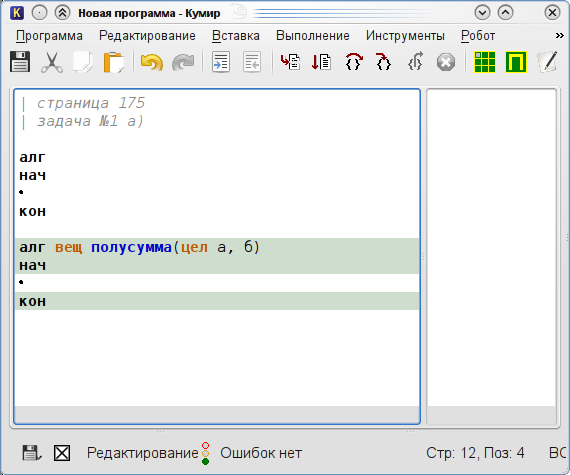
\includegraphics[scale=1]{ctrl_t_figure1.png}
\caption{Программа с заготовками вспомогательного алгоритма}
\end{center}
\end{figure}

Строки, выделенные темным фоном, защищены от изменения. Это значит, что имя алгоритма и список его параметров заданы заранее, и их нельзя поменять.
Для выполнения задания нужно написать тело вспомогательного алгоритма и убедиться в правильности его работы, подготовив и выполнив соответствующий основной алгоритм.

\begin{figure}[htb]
\begin{center}
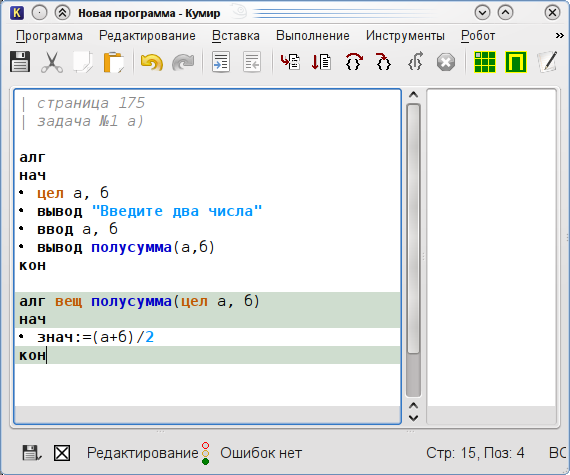
\includegraphics[scale=1]{ctrl_t_figure2.png}
\caption{Реализация программы учеником}
\end{center}
\end{figure}

\subsection{Тестовый алгоритм}

В задание включен также алгоритм тестирования вспомогательного алгоритма, подготовленного учащимся. Этот алгоритм  по желанию учителя может быть скрыт от ученика (как на показано на предыдущих двух рисунках) или виден ему:

\begin{figure}[htb]
\begin{center}
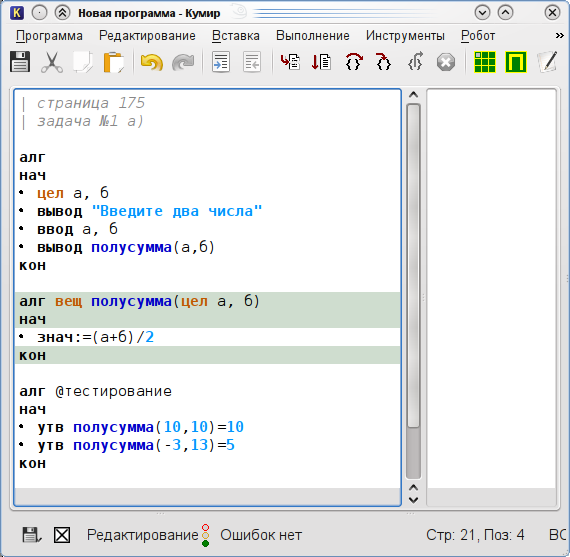
\includegraphics[scale=1]{ctrl_t_figure3.png}
\caption{Тестирующий алгоритм \texttt{@тестирование}}
\end{center}
\end{figure}

После того, как вспомогательный алгоритм будет готов, полученную программу можно проверить. Для этого необходимо выбрать пункт меню \textsc{Программа}$\rightarrow$\textsc{Запустить} 
\textsc{тестирование} либо нажать комбинацию клавиш \textsc{Ctrl+T}. 
Эти действия приводят к выполнению алгоритма с именем \texttt{@тестирование}.

Тестирование может завершиться с двумя исходами:
Если ошибок не обнаружено, то после окончания тестирования в поле ввода-вывода запишется строка \lq\lq Тестирование завершено успешно\rq\rq.
Если в процессе выполнения тестирующего алгоритма произойдет ошибка (это означает, что есть ошибка 
в алгоритме ученика), то тестирование прервется с сообщением \lq\lq Ошибка выполнения тестирования\rq\rq.


Возможна ситуация, когда в заготовке программы не предусмотрена возможность тестирования. В этом случает при выборе пункта 
меню  \textsc{Программа}$\rightarrow$\textsc{Запустить} \textsc{тестирование} либо 
при нажатии комбинации клавиш \textsc{Ctrl+T} появится сообщение \lq\lq Программа не содержит тестирующего алгоритма\rq\rq.

\section{Гипертекстовый учебник}

В состав поставки \textsc{КуМир} входит гипертекстовый учебник, тесно взаимодействующий с системой. Этот учебник можно использовать с
помощью Web-браузера. Вызовы гипертекстового учебника производится из меню \textsc{Инструменты}$\rightarrow$\textsc{Гипертекстовый учебник}.

\textbf{Замечание.} В настоящее время текст данного учебника находится в стадии разработки.
